\documentclass[handouts]{beamer}
\usepackage[orientation=portrait,size=a4, scale=2]{beamerposter}
\beamertemplatenavigationsymbolsempty

\usepackage[czech]{babel}
\usepackage{booktabs}

\title{Maticové modely v ekologii}
\author{Robert Mařík}
\usetheme{CambridgeUS}
\usecolortheme{crane}

\def\subsection#1{\par\medskip \textbf{#1}\par\medskip}
\begin{document}

\begin{frame}

  \vskip 0 pt plus 1 filll
  
  \begin{center}
    \large Maticové modely v ekologii
  \end{center}

  \vskip 0 pt plus 1 filll


  \begin{block}{Maticový přístup k modelování populací}
    Mnoho populací či systémů splňuje následující předpoklady.
  \begin{itemize}
  \item Členové populace jsou rozděleni do tříd. Například podle věku,
    vývojového stadia apod. Podobně mohou být rozděleny složky
    ekosystému do tříd podle druhu dominantního porostu apod.
  \item Členové jednotlivých tříd v dalším období s danými pravděpodobnostmi buď zůstávají ve své třídě nebo ji mění.
  \item Počet členů každé třídy v dalším období se stanoví jako součet příspěvků ze všech tříd.    
  \end{itemize}
\end{block}

\begin{exampleblock}{Model populace tuleňů (Monagan, Using Leslie matrices as the application \dots (2020))}
  \begin{columns}
    \begin{column}[t]{0.6\hsize}
  Populace samiček tuleňů je rozdělena na tři třídy: mláďata (0 až 4
  roky), mladé tuleně (4 až 8 let) a dospělé tuleně (nad 8
  let). Jednotka času jsou 4 roky.
  \begin{itemize}
  \item Mláďata do čtyř let nemají
  potomky. 
\item Mladí tuleni mají průměrně $1.26$ a dospělí průměrně $2.0$
  samičích potomků každé 4 roky. 
\item Mláďata dorostou do další věkové
  kategorie (tj. nezahynou) s pravděpodobností 0.614. 
\item Mladí tuleni
  dorostou do kategorie dospělých s pravděpodobností 0.808 a
  pravděpodobnost, že starý tuleň přežije další 4 roky je také 0.808.
\end{itemize}

\end{column}
\begin{column}[t]{0.38\hsize}
  Je-li $x_i(t)$ velikost $i$-té kategorie v čase $t$, je možné
  reprezentovat model rekurentním vztahem tvořeným následující
  soustavou rovnic.

  \begin{equation*}
    \begin{alignedat}{4}
    x_1(t+1) &= &&1.26 x_2(t) + 2.0 x_3(t)\\
    x_2(t+1) &= 0.614&& x_1(t)\\
    x_3(t+1) &= &&0.808 x_2(t) + 0.808 x_3(t)\\
  \end{alignedat}
  \end{equation*}
\end{column}
\end{columns}
\end{exampleblock}

\begin{columns}

  \begin{column}[t]{0.5\hsize}
Pro práci se systémy uvedeného typu ale libovolné složitosti co se
týká počtu proměnných i vnitřních vazeb je vhodnější nepracovat s rekurentní soustavou rovnic, ale stav systému reprezentovat pomocí
vektorů a koeficienty pomocí \textbf{matice}. V tomto smyslu se jedná o projekci vektoru pomocí \textbf{projekční matice} do nového časového období. Matematicky
tuto operaci nazýváme \textbf{součin matice a vektoru}.
\end{column}


  \begin{column}[t]{0.48\hsize}
\begin{exampleblock}{Maticový model}
Model populace tuleňů v maticovém tvaru je
$$\begin{pmatrix} x_1(k+1) \\ x_2(k+1) \\ x_3 (k+1) \end{pmatrix} = \begin {pmatrix}   0  &1.26&2.0\cr 0.614&0&0&\cr 0&0.808&0.808 \end{pmatrix} \begin{pmatrix} x_1(k) \\ x_2(k) \\  x_3 (k) \end{pmatrix}.$$
\end{exampleblock}

\end{column}
\end{columns}

\vskip 0 pt plus 1 filll
%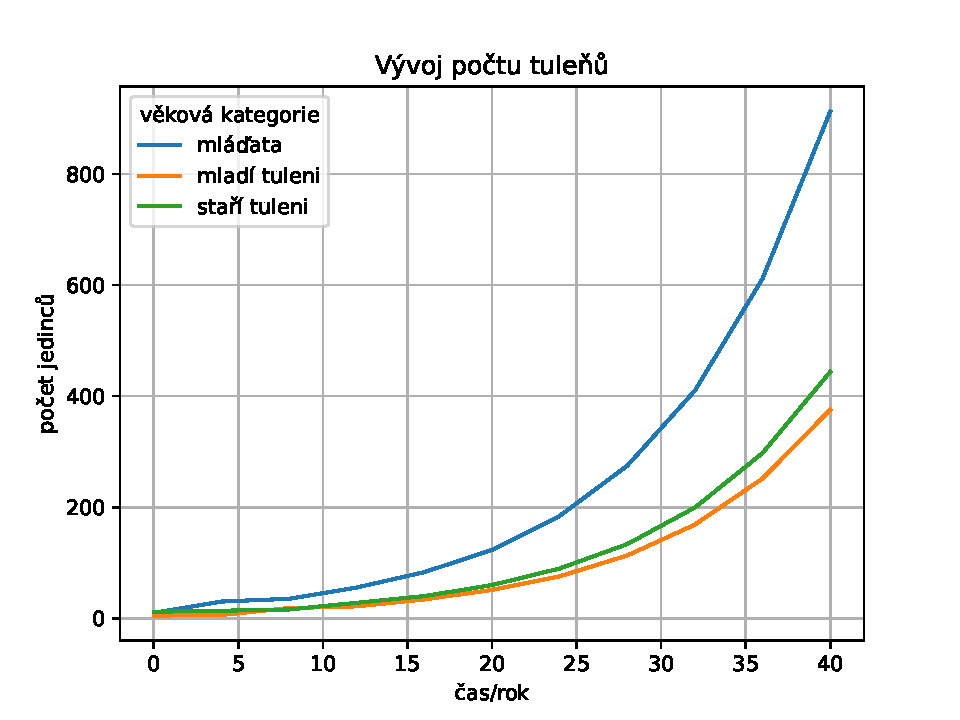
\includegraphics{tuleni.pdf}
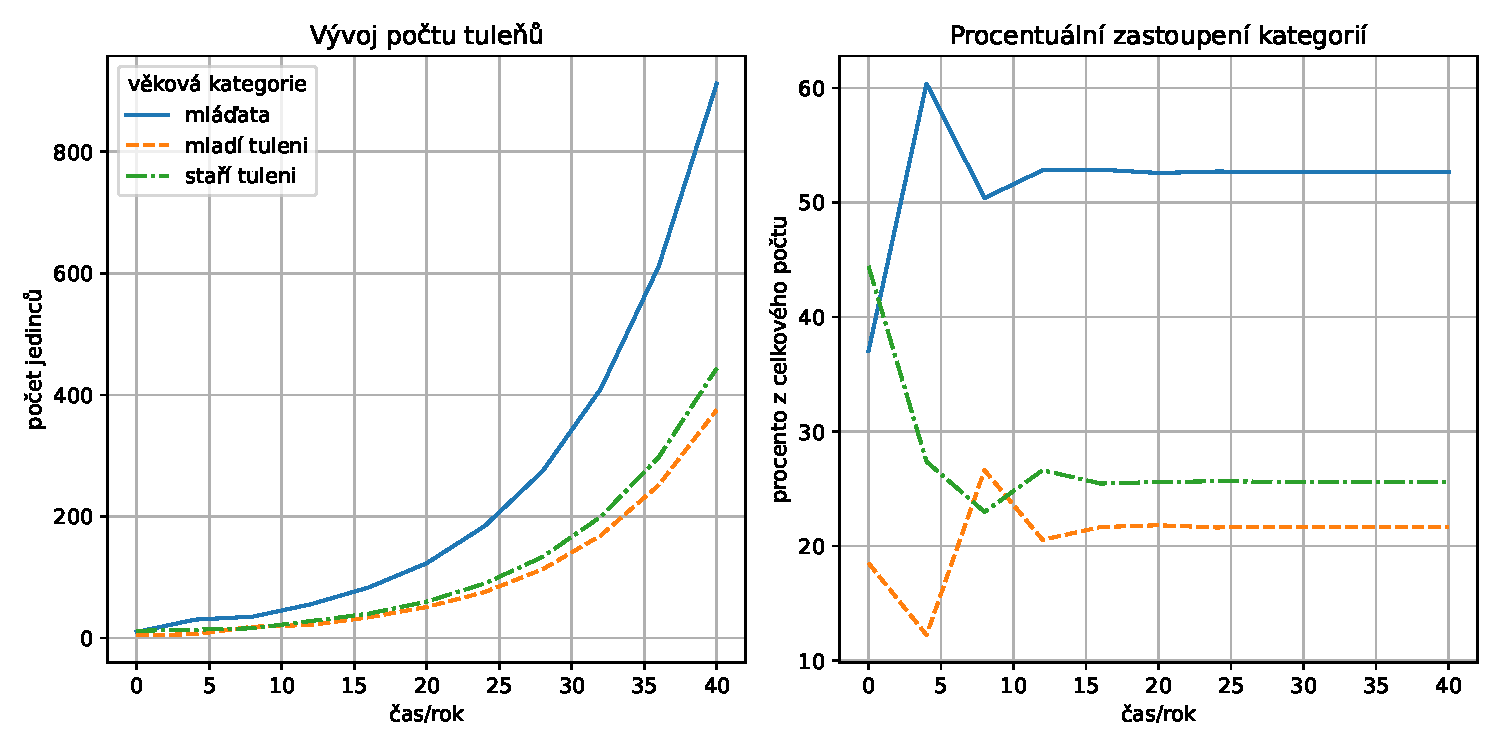
\includegraphics[width=\linewidth]{tuleni2.pdf}

\end{frame}
\end{document}


%%% Local Variables: 
%%% TeX-command-extra-options: "-shell-escape"
%%% TeX-engine: xetex
%%% End:
